
\section{Iterative description}
\label{sec:description}

In the appendix of his PhD thesis, Gaunce Lewis Jr. \cite[p.~158]{Le78} makes explicit the least drastic way of transforming a $k$-space into a compactly generated space, which is (defined as) a space that is both a $k$-space and a weak Hausdorff space. Lewis describes an iterative process. At each stage of the process, two points are identified whenever it is impossible to separate them by (disjoint) open sets.

We will provide an iterative description of the process of forming $UDX$ from $X$ that is analogous to Lewis' method. In the least drastic way possible, we want to make a quotient of $X$ so that the vertices of any non-degenerate simplex are pairwise distinct. In other words, any non-degenerate simplex of $X$ whose vertices are not pairwise distinct, must be made degenerate. For this purpose, we will use the notion of enforcer from \cref{def:enforcer}.

In relation to \cref{thm:main_result_itdesing}, there is a systematic study of reflective subcategories provided by S. Baron \cite{Ba69}. First, $nsSet$ is epi-reflective as the map $X\to DX$ is epic in general. Second, Baron discusses the possibility of factoring the reflector through a unique intermediate category.

In the following way, we define a functor $J:sSet\to sSet$ together with a natural quotient map $X\to JX$ that $\eta _X$ factors through. The functor $J$ is thought of as a preferred first step towards making a simplicial set non-singular. We have taken the symbol $J$ because Lewis uses it to denote his analogous endofunctor of $k$-spaces.

Let $X$ be a simplicial set. Given a non-degenerate simplex $x$ of $X$, we let $n_x$ denote its degree. Recall the enforcer $\rho _x:[n_x]\to [m_x]$ of $x$ from \cref{def:enforcer}. We will construct a cobase change of
\[A=\bigsqcup _{x\in X^\sharp}\Delta [n_x]\xrightarrow{f=\sqcup _{x\in X^\sharp }(\rho _x)} \bigsqcup _{x\in X^\sharp}\Delta [m_x]=B\]
along
\[A\xrightarrow{g=\vee _{x\in X^\sharp }(\bar{x} )} X.\]
The latter map is degreewise surjective as $X^\sharp$ generates $X$.

For each integer $n\geq 0$, define a symmetric binary relation $R'_n$ on $X_n$ by letting $(x,x')\in X_n\times X_n$ be a member of a set $R'_n$ if there are $a,a'\in A_n$ such that
\begin{displaymath}
\begin{array}{rcl}
x & = & g(a) \\
x' & = & g(a') \\
f(a) & = & f(a').
\end{array}
\end{displaymath}
The binary relation $R'_n$, $n\geq 0$, is reflexive as $g$ is degreewise surjective.

Let $R_n$ be the equivalence relation generated by $R'_n$, for each $n$. It follows immediately that the equivalence relations $R_n$, $n\geq 0$, satisfy the condition that the diagrams (\ref{eq:first_diagram_proof_lem_desing_unique_factorization_through_unit}) commute. This implies that we can form the quotient
\[JX=X/R.\]
Thus we obtain the cocartesian square
\begin{displaymath}
 \xymatrix{
 \bigsqcup _{x\in X^\sharp}\Delta [n_x] \ar[d]_{\vee _{x\in X^\sharp }(\bar{x} )} \ar[rr]^{\sqcup _{x\in X^\sharp }(\rho _x)} && \bigsqcup _{x\in X^\sharp}\Delta [m_x] \ar[d] \\
 X \ar[rr] && JX
 }
\end{displaymath}
in $sSet$. By \cref{lem:pushout_along_enforcers_intermediate_desingularization}, it gives rise to a commutative triangle
\begin{equation}
\label{eq:first_diagram_description_iterative}
\begin{gathered}
\xymatrix{
X \ar[dr]_{\eta _X} \ar[rr] && JX \ar[ld] \\
& UDX
}
\end{gathered}
\end{equation}
that factors the unit $\eta _X$ through a quotient map $X\to JX$, which is the identity in the case when $X$ is already non-singular.

For the purposes of making an iterative description of desingularization, the notation above is suitable. However, the construction $JX$ deserves its own name.
\begin{definition}\label{def:enforced_collapse}
Let $X$ be a simplicial set. The map $X\to JX$ is the \textbf{enforced collapse} of $X$.
\end{definition}
\noindent Outside of the context of the iteration process below we may choose to use the following symbol
\begin{notation}
Let $X$ be a simplicial set. Let
\[Cen(X)=JX\]
denote the enforced collapse of $X$.
\end{notation}
\noindent Note that the enforced collapse need not be non-singular, as \cref{ex:infinitely_many_enforced_collapses_needed} shows.
\begin{example}\label{ex:infinitely_many_enforced_collapses_needed}
Consider the $2$-dimensional simplicial set depicted in \cref{fig:ch2_finite_number_of_enforced_collapses_not_enough}. Identify the two $0$-simplices $v$ and $w$. The result can be constructed thus.

Let
\[\mathbb{N} =\{ 1,2,\dots \}\]
and
\[\mathbb{N} _0=\{ 0,1,2,\dots \} .\]
Next, for each $n\in 2\mathbb{N}$, let $B_n=\Delta [2]$. For each $n\in \mathbb{N} _0$, let $A_n=\Delta [1]$. Furthermore, let $C_0=\Delta [1]/\partial \Delta [1]$. Finally, for each $n\in \mathbb{N}$, let $C_n=\Delta [1]$.

Take the pushout $X$ in $sSet$ of
\begin{equation}
\label{eq:first_diagram_ex_infinitely_many_enforced_collapses_needed}
\begin{gathered}
\xymatrix{
\bigsqcup _{n\in \mathbb{N} _0}A_n \ar[d] \ar[r] & \bigsqcup _{n\in 2\mathbb{N} _0}C_n \\
\bigsqcup _{n\in 2\mathbb{N} }B_n
}
\end{gathered}
\end{equation}
where the maps are defined as follows. Let $X$ denote the pushout.

Suppose $n\in \mathbb{N} _0$. In the case when $n\equiv 0\; (mod\, 4)$, we let $A_n\to B_{n+2}$ be the map induced by $\delta _1$ and we let $A_{n+1}\to B_{n+2}$ be the map induced by $\delta _2$. In the case when $n\equiv 2\; (mod\, 4)$, we let $A_n\to B_{n+2}$ be the map induced by $\delta _1$ and we let $A_{n+1}\to B_{n+2}$ be the map induced by $\delta _0$. These maps give rise to the map
\[\bigsqcup _{n\in \mathbb{N} _0}A_n\to \bigsqcup _{n\in 2\mathbb{N} }B_n\]
in (\ref{eq:first_diagram_ex_infinitely_many_enforced_collapses_needed}).

Let $A_0\to C_0$ be the canonical map. Suppose $n\in \mathbb{N} _0$ odd. Then we let $A_n\to C_{n+1}$ and $A_{n+1}\to C_{n+1}$ be the identity $\Delta [1]\to \Delta [1]$. These maps give rise to the map
\[\bigsqcup _{n\in \mathbb{N} _0}A_n\to \bigsqcup _{n\in 2\mathbb{N} _0}C_n\]
in (\ref{eq:first_diagram_ex_infinitely_many_enforced_collapses_needed}).

If $Cen^k$ denotes the $k$-fold iteration of the enforced collapse for $k$ a non-negative integer, then $Cen^k(X)$ is singular for every $k$.
\end{example}
\noindent \cref{ex:infinitely_many_enforced_collapses_needed} shows that one might need an infinite number of enforced collapses in order to make a simplicial set non-singular.

\begin{figure}
\centering
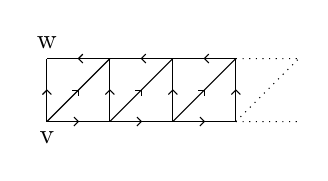
\begin{tikzpicture}[scale=0.4]

% $0$-simplices coordinates
\coordinate (0) at (-5,-1);
\coordinate (2) at (-3,-1);
\coordinate (4) at (-1,-1);
\coordinate (6) at (1,-1);

\coordinate (1) at (-5,1);
\coordinate (3) at (-3,1);
\coordinate (5) at (-1,1);
\coordinate (7) at (1,1);


% Nodes to aid in the drawing process
\node [below] at (0) {v};
% \node [below] at (2) {2};
% \node [below] at (4) {4};
% \node [below] at (6) {6};

\node [above] at (1) {w};
% \node [above] at (3) {3};
% \node [above] at (5) {5};
% \node [above] at (7) {7};


% $1$-simplices drawn
\draw (0.north)--(1.south) coordinate[midway](01);
\draw (2.north)--(3.south) coordinate[midway](23);
\draw (4.north)--(5.south) coordinate[midway](45);
\draw (6.north)--(7.south) coordinate[midway](67);

\draw (0.north)--(3.south) coordinate[midway](03);
\draw (2.north)--(5.south) coordinate[midway](25);
\draw (4.north)--(7.south) coordinate[midway](47);
\draw [dotted] (6.north)--(3,1);

\draw (0.north)--(2.north) coordinate[midway](02);
\draw (2.north)--(4.north) coordinate[midway](24);
\draw (4.north)--(6.north) coordinate[midway](46);
\draw [dotted] (6.north)--(3,-1);

\draw (1.south)--(3.south) coordinate[midway](13);
\draw (3.south)--(5.south) coordinate[midway](35);
\draw (5.south)--(7.south) coordinate[midway](57);
\draw [dotted] (7.south)--(3,1);

% Directions
\draw (01)--+(225:0.2cm);
\draw (01)--+(315:0.2cm);

\draw (23)--+(225:0.2cm);
\draw (23)--+(315:0.2cm);

\draw (45)--+(225:0.2cm);
\draw (45)--+(315:0.2cm);

\draw (67)--+(225:0.2cm);
\draw (67)--+(315:0.2cm);


\draw (02)--+(135:0.2cm);
\draw (02)--+(225:0.2cm);

\draw (24)--+(135:0.2cm);
\draw (24)--+(225:0.2cm);

\draw (46)--+(135:0.2cm);
\draw (46)--+(225:0.2cm);


\draw (13)--+(45:0.2cm);
\draw (13)--+(315:0.2cm);

\draw (35)--+(45:0.2cm);
\draw (35)--+(315:0.2cm);

\draw (57)--+(45:0.2cm);
\draw (57)--+(315:0.2cm);


\draw (03)--+(180:0.2cm);
\draw (03)--+(270:0.2cm);

\draw (25)--+(180:0.2cm);
\draw (25)--+(270:0.2cm);

\draw (47)--+(180:0.2cm);
\draw (47)--+(270:0.2cm);
\end{tikzpicture}
\caption{Simplicial set such that every finite iteration of enforced collapses is singular.}
\label{fig:ch2_finite_number_of_enforced_collapses_not_enough}
\end{figure}

We point out the following, which is not really part of the storyline.
\begin{remark}\label{rem:description_iterative}
The map $\vee _{x\in X^\sharp }(\bar{x} )$ is degreewise surjective because $X^\sharp$ generates $X$. In this way, the construction of the functor $J$ is less arbitrary than the setting in \cref{lem:pushout_along_enforcers_intermediate_desingularization}.

One can, however, replace $X^\sharp$ with a subset and still construct symmetric binary relations $R'_n$, $n\geq 0$, the same way. Each of them is reflexive if and only if the subset generates $X$. We can in either case choose a quotient map as the cobase change of $\sqcup _{x\in X^\sharp }(\rho _x)$ along $\vee _{x\in X^\sharp }(\bar{x} )$.

For example, in the proof of \cref{prop:double_subdivision_sphere_low_dimension}, or more specifically the diagram (\ref{eq:second_diagram_proof_prop_double_subdivision_sphere_low_dimension}), we did choose a suitable subset of the set of non-degenerate simplices to perform a desingularization.
\end{remark}
\noindent \cref{rem:description_iterative} might be useful in some cases as suggested by the proof of \cref{prop:double_subdivision_sphere_low_dimension}.

To define $J$ on morphisms $f:X\to Y$ we need a diagram of the form
\begin{equation}
\label{eq:second_diagram_description_iterative}
\begin{gathered}
 \xymatrix{
 X \ar[d]_f & \bigsqcup _{x\in X^\sharp}\Delta [n_x] \ar[l] \ar[d] \ar[r] & \bigsqcup _{x\in X^\sharp}\Delta [m_x] \ar@{-->}[d] \\
 Y & \bigsqcup _{y\in Y^\sharp}\Delta [n_y] \ar[l] \ar[r] & \bigsqcup _{y\in Y^\sharp}\Delta [m_y]
 }
\end{gathered}
\end{equation}
in which an obvious choice of middle vertical map is $f(x)^\flat$ for each index $x\in X^\sharp$. Here, we write $f(x)=f(x)^\sharp f(x)^\flat$ by means of the Eilenberg-Zilber lemma.

There is at most one dashed map that makes the square
\begin{equation}
\label{eq:third_diagram_description_iterative}
\begin{gathered}
 \xymatrix{
 [n_x] \ar[d]_{f(x)^\flat } \ar[r]^{\rho _x} & [m_x] \ar@{-->}[d] \\
 [n_{f(x)^\sharp }] \ar[r]_{\rho _{f(x)^\sharp }} & [m_{f(x)^\sharp }]
 }
\end{gathered}
\end{equation}
commute as $\rho _x$. We claim that if $\mu _x$ is a section of $\rho _x$, then
\[\rho _{f(x)\sharp }\circ f(x)^\flat \circ \mu _x\]
makes the square commute. This claim holds if
\begin{equation}\label{eq:first_equation_description_iterative}
\rho _{f(x)^\sharp }\circ f(x)^\flat (i)=\rho _{f(x)^\sharp }\circ f(x)^\flat (j)
\end{equation}
whenever
\begin{equation}\label{eq:second_equation_description_iterative}
\rho _x(i)=\rho _x(j).
\end{equation}
If the claim holds, then any other section of $\rho _x$ would yield the same functor $[k_x]\to [k_{f(x)^\sharp }]$. From dashed maps that makes the diagrams (\ref{eq:third_diagram_description_iterative}) commute, we get a dashed map that makes (\ref{eq:second_diagram_description_iterative}) commute. With it arises a map $J(f)$.

Now we argue that (\ref{eq:first_equation_description_iterative}) holds whenever (\ref{eq:second_equation_description_iterative}) does. The degeneracy operator $\rho _x$ corresponds to the equivalence relation on $[n_x]$ that is generated by the reflexive binary relation $\approx$ that is defined in \cref{sec:calculations}. Hence, our claim will follow if $i\approx k$ implies that
\begin{equation}\label{eq:third_equation_description_iterative}
\rho _{f(x)^\sharp }\circ f(x)^\flat (i)=\rho _{f(x)^\sharp }\circ f(x)^\flat (k)
\end{equation}
holds.

Suppose $x\varepsilon _i=x\varepsilon _j$. This implies $f(x)\varepsilon _i=f(x)\varepsilon _j$, which can be rewritten as
\[f(x)^\sharp f(x)^\flat \varepsilon _i=f(x)^\sharp f(x)^\flat \varepsilon _j,\]
which in turn can be rewritten as
\[f(x)^\sharp \varepsilon _{f(x)^\flat (i)}=f(x)^\sharp \varepsilon _{f(x)^\flat (j)}.\]
By definition of $\rho _{f(x)^\sharp }$ it follows that
\[\rho _{f(x)^\sharp }(f(x)^\flat (i))=\rho _{f(x)^\sharp }(f(x)^\flat (j)).\]
Next, suppose $i\leq k\leq j$. In other words, we assume $i\approx k$. Degeneracy operators are order-preserving, so (\ref{eq:third_equation_description_iterative}) holds. This concludes our definition of $J(f)$.

It is clear that $J(id)=id$, for in the case $f=id$ we have that $f(x)^\flat =id$ and $\rho _x=\rho _{f(x)^\sharp }$. It follows that
\[J(g\circ f)=J(g)\circ J(f)\]
from the fact that the square
\begin{displaymath}
\xymatrix{
X \ar[d] \ar[r]^f & Y \ar[d] \\
JX \ar[r]_{J(f)} & JY
}
\end{displaymath}
commutes for each simplicial map $f:X\to Y$ combined with the fact that $X\to JX$ is degreewise surjective for each simplicial set $X$. Thus the construction $JX$ is functorial and the map $X\to JX$ is natural. Because $X\to JX$ is natural and degreewise surjective and because $\eta _X$ is natural, it follows that $JX\to UDX$ is natural.

The plan is to obtain a quotient of $X$ that is isomorphic to $UDX$ by applying $J$ successively. Moreover, we aim to establish \cref{thm:main_result_itdesing}. To arrange for the iteration, we refer to \cref{def:sequence_composition}. Let $f^{0,1}$ be the natural map
\[J^0X=X\to JX=J^1X.\]
Due to (\ref{eq:first_diagram_description_iterative}), we can assume that we for some ordinal $\gamma >1$ have defined a $\gamma$-sequence
\[T^{[0]}\Rightarrow \cdots \Rightarrow T^{[\beta ]}\Rightarrow T^{[\beta +1]}\Rightarrow \cdots\]
of commutative triangles
\begin{equation}
\label{eq:fourth_diagram_description_iterative}
\begin{gathered}
\xymatrix{
X \ar[dr]_{\eta _X} \ar[rr] && J^\beta X \ar[ld]^{p^\beta} \\
& UDX
}
\end{gathered}
\end{equation}
denoted $T^{[\beta ]}$ and natural transformations, in which the component
\[J^\alpha X\xrightarrow{f^{\alpha ,\beta }} J^\beta X\]
of $T^{[\alpha ]}\Rightarrow T^{[\beta ]}$ is a quotient map whenever $\alpha \leq \beta <\gamma$.

If $\gamma$ is a limit ordinal, then we take the colimit in the following way to define $J^\gamma X$. For each $n\geq 0$, let $R_n$ be the equivalence relation on $J^0X=X$ that consists of the elements $(x,y)\in X_n\times X_n$ such that there is some $\beta <\gamma$ with $f^{0,\beta }(x)=f^{0,\beta }(y)$. It is clear that the diagrams (\ref{eq:first_diagram_proof_lem_desing_unique_factorization_through_unit}) commute so that we obtain the quotient $J^\gamma X=X/R$ of $J^0X$. In this case, we automatically get a diagram $T^{[\gamma ]}$ that plays the role of (\ref{eq:fourth_diagram_description_iterative}).

Else if $\gamma =\beta +1$ is a successor of an ordinal $\beta$, then we simply define $J^{\beta +1}X$ by applying $J$ to $J^\beta X$. Consider the solid commutative diagram
\begin{equation}
\label{eq:fifth_diagram_description_iterative}
\begin{gathered}
\xymatrix{
X \ar[dd]_{id} \ar[dr]_{\eta _X} \ar[rr] && J^\beta X \ar[ld]^{p^\beta } \ar[dd]^{f^{\beta ,\beta +1}} \\
& UDX \ar[dd]_(.65){id} \\
X \ar[dr]_{\eta _X} \ar@{-}[r] & \ar[r] & J^{\beta +1}X \ar@{-->}[ld]^{p^{\beta +1}} \\
& UDX
}
\end{gathered}
\end{equation}
in which we have yet to define the dashed map $p^{\beta +1}$. By \cref{prop:role_of_enforcers}, we obtain the dashed map in the solid diagram
\begin{equation}
\label{eq:sixth_diagram_description_iterative}
\begin{gathered}
\xymatrix{
& \bigsqcup _{j\in (J^\beta X)^\sharp}\Delta [n_j] \ar[dd]_{\vee _{j\in (J^\beta X)^\sharp }(\bar{\jmath } )} \ar[rr]^{\sqcup _{j\in (J^\beta X)^\sharp }(\rho _j)} && \bigsqcup _{j\in (J^\beta X)^\sharp}\Delta [m_j] \ar[dd] \\
\\
X \ar[d]_\eta \ar[r]^{f^{0,\beta }} & J^\beta X \ar[ld]^(.45){p^\beta } \ar[d]^\eta \ar[rr]^{f^{\beta ,\beta +1}} && J^{\beta +1}X \ar@{-->}[lld] \ar[d]^\eta \\
UDX \ar[r]_(.45){UD(f^{0,\beta })} & UD(J^\beta X) \ar[rr]_{UD(f^{\beta ,\beta +1})} && UD(J^{\beta +1})
}
\end{gathered}
\end{equation}
in $sSet$, which commutes because $f^{0,\beta }$ is a quotient map and hence degreewise surjective.

The whole diagram (\ref{eq:sixth_diagram_description_iterative}) commutes because $f^{\beta ,\beta +1}$ is degreewise surjective. This implies that $UD(f^{0,\beta })$ and $UD(f^{\beta ,\beta +1})$ are isomorphisms. Hence, from (\ref{eq:sixth_diagram_description_iterative}) we obtain a canonical dashed map $p^{\beta +1}$ in (\ref{eq:fifth_diagram_description_iterative}) that makes the whole diagram commute, including the lower triangle.

We have finished the construction of a $\gamma$-sequence $T:\gamma \to sSet^{[2]}$ for each ordinal $\gamma$. By the design of these sequences, there is a canonical composition of each of them that is a quotient map.

Next, we verify that this iterative process does indeed come to a halt. The proof uses the following observation.
\begin{lemma}\label{lem:no_break_iterative_desingularization}
If $\beta$ is some ordinal and if some $x\in (J^\beta X)^\sharp$ is not embedded, then $f^{\beta ,\beta +1}(x)$ is a degenerate simplex in $J^{\beta +1}X$.
\end{lemma}
\begin{proof}
Consider the diagram
\begin{equation}
\label{eq:first_diagram_proof_lem_no_break_iterative_desingularization}
\begin{gathered}
\xymatrix@=0.7em{
\Delta [n_x] \ar[dd] \ar[rr]^{\rho _x} && \Delta [m_x] \ar@/_1.9pc/[lddd] \ar[dd] \\
\\
\bigsqcup _{j\in (J^\beta X)^\sharp }\Delta [n_j] \ar[dd]_{\vee _{j\in (J^\beta X)^\sharp }{(\bar{\jmath } )}} \ar@{-}[r] & \ar[r] & \bigsqcup _{j\in (J^\beta X)^\sharp }\Delta [m_j] \ar[dd] \\
& Y \ar@{-->}[dr] \\
J^\beta X \ar[ur] \ar[rr]_{f^{\beta ,\beta +1}} && J^{\beta +1}X
}
\end{gathered}
\end{equation}
where we take the pushout
\[Y=J^\beta X\sqcup _{\Delta [n_x]}\Delta [m_x].\]
The quotient map $f^{\beta ,\beta +1}X$ factors through the canonical map $J^\beta X\to Y$. The map $Y\to J^{\beta +1}X$ is then also degreewise surjective. To say that $x$ is not embedded is the same as saying that its vertices are not pairwise distinct, so $\rho _x$ is a proper degeneracy operator. Thus we see that
\[\Delta [n_x]\xrightarrow{\bar{x} } J^\beta X\to Y\]
is the representing map of a degenerate simplex. To precompose this representing map with $Y\to J^{\beta +1}X$ yields the map $f^{\beta ,\beta +1}\circ \bar{x}$, as we see from (\ref{eq:first_diagram_proof_lem_no_break_iterative_desingularization}). It follows that $f^{\beta ,\beta +1}(x)$ is degenerate.
\end{proof}
\begin{proposition}\label{prop:iterative_desingularization_halts}
Let $X$ be a simplicial set. There is an ordinal $\lambda$ such that $J^\lambda X$ is non-singular.
\end{proposition}
\begin{corollary}\label{cor:iterative_desingularization_halts}
Let $X$ be a simplicial set. There is an ordinal $\lambda$ such that the map
\[p^\lambda :J^\lambda X\xrightarrow{\cong } UDX\]
is an isomorphism.
\end{corollary}
\begin{proof}[Proof of \cref{cor:iterative_desingularization_halts}.]
Use \cref{prop:iterative_desingularization_halts} to choose an ordinal $\kappa$ such that $J^\kappa X$ is non-singular.

According to \cref{lem:pushout_along_enforcers_intermediate_desingularization}, the canonical map $J^{\kappa +1}X\xrightarrow{\cong } UD(J^\kappa X)$ is an isomorphism as $J^{\kappa +1}X$ is non-singular, which is in turn because $f^{\kappa ,\kappa +1}$ is the identity. Recall the successor ordinal step from the construction of $T$ and replace $\beta$ with $\kappa$ in the diagram (\ref{eq:sixth_diagram_description_iterative}).

As $f^{\kappa ,\kappa +1}$ is the identity, it follows that the isomorphism above is in fact equal to $\eta _{J^\kappa X}$. The map $J^{\kappa +1}X\to UDX$ is by design equal to the composite
\[J^{\kappa +1}X=J^\kappa X\xrightarrow{\eta _{J^\kappa X}} UD(J^\kappa X)\to UDX.\]
The first half $\eta _{J^\kappa X}$ of the composite above is an isomorphism by the choice of $\kappa$ and the second half is the inverse of
\[UD(f^{0,\kappa }):UDX\to UD(J^\kappa X)\]
If we define $\lambda =\kappa +1$, then the proof is finished.
\end{proof}
\begin{proof}[Proof of \cref{prop:iterative_desingularization_halts}.]
The idea of the proof is that we can index the simplicial sets $J^\beta X$ that are singular by a certain subset of the non-degenerate simplices of $X$.

If $J^0X=X$ is already non-singular, then we can let $\lambda =0$. Else if $X$ is singular, then we choose a non-embedded non-degenerate simplex $x^0$ of $X$. Suppose $\gamma >0$ is such that we for all $\beta$ with $\beta <\gamma$ have defined $x^\beta$ with $x^\alpha \neq x^\beta$ if $\alpha <\beta <\gamma$.

If $J^\gamma X$ is non-singular, then we define $\lambda =\gamma$. Else if $J^\gamma X$ is singular, then we choose a simplex $x^\gamma$ of $X$ such that $f^{0,\gamma }(x^\gamma )$ is a non-embedded non-degenerate simplex. Suppose $\beta$ an ordinal with $\beta <\gamma$. From the commutative diagram
\begin{equation}
\label{eq:first_diagram_proof_prop_iterative_desingularization_halts}
\begin{gathered}
 \xymatrix{
 X \ar[dr]_{f^{0,\beta }} \ar[rr]^{f^{0,\gamma }} && J^\gamma X \\
 & J^\beta X \ar[ur]^{f^{\beta ,\gamma }} \ar[rr]_{f^{\beta ,\beta +1}} && J^{\beta +1}X \ar[lu]_{f^{\beta +1,\gamma }}
 }
 \end{gathered}
\end{equation}
we will conclude that
\begin{equation}\label{eq:first_equation_proof_prop_iterative_desingularization_halts}
x^\beta \neq x^\gamma
\end{equation}
in the following way.

Define
\begin{displaymath}
\begin{array}{rcl}
y & = & f^{0,\beta }( x^\beta) \\
y' & = & f^{\beta ,\beta +1}(y) \\

\end{array}
\end{displaymath}
As $y'$ is degenerate by \cref{lem:no_break_iterative_desingularization}, it follows that $f^{\beta +1,\gamma }(y')$ is degenerate. Because the diagram (\ref{eq:first_diagram_proof_prop_iterative_desingularization_halts}) commutes, this simplex is equal to
\[f^{\beta +1,\gamma }(y')=f^{\beta ,\gamma }(y)=f^{0,\gamma }(x^\beta ).\]
On the other hand, the simplex $f^{0,\gamma }(x^\gamma )$ is non-degenerate, so, as announced, it follows that (\ref{eq:first_equation_proof_prop_iterative_desingularization_halts}) holds.

Let $\lambda$ be a cardinal that is strictly greater than the cardinality of $X^\sharp$. Define $S$ as the set consisting of those $x^\beta$ with $\beta \leq \lambda$. This is a subset of $X^\sharp$. Then we can consider the injective function $S\to \lambda +1$ defined by $x^\beta \mapsto \beta$. If $\alpha <\beta$, then $x^\alpha$ is defined if $x^\beta$ is. In other words, $\alpha$ is in the image of $S\to \lambda +1$ if $\beta$ is.

By the choice of $\lambda$, there does not exist a surjective extension
\begin{displaymath}
\xymatrix{
S \ar[dd] \ar[dr] \\
& \lambda +1 \\
X^\sharp \ar@{-->>}[ur]_\nexists
}
\end{displaymath}
of $S\to \lambda +1$ to $X^\sharp$. Therefore, the function $S\to \lambda +1$ cannot possibly be surjective. Hence, the element $\lambda$ is not in the image of the latter function. By the definition of $S$, it follows that $x^\lambda$ is not defined. This implies that the set $S$ contains every element in $X^\sharp$ with a designation $x^\beta$. This shows that $J^\lambda X$ is non-singular.
\end{proof}
\begin{proof}[Proof of \cref{thm:main_result_itdesing}.]
Use \cref{cor:iterative_desingularization_halts} to choose an ordinal $\lambda$ such that $p^\lambda$ is an isomorphism. Take the corresponding $\lambda$-sequence $T$ of triangles (\ref{eq:fourth_diagram_description_iterative}) from the family of sequences constructed above. The map $f^{0,\lambda }$ is the composition of the $\gamma$-sequence
\[J^0X\xrightarrow{f^{0,1}} \cdots \to J^\beta X\xrightarrow{f^{\beta ,\beta +1}} \cdots\]
by the design of $J^{\lambda +1}$. Because $p^\lambda$ is an isomorphism, the commutative triangle $T^{[\lambda ]}$ identifies $f^{0,\lambda }$ with $\eta _X$.
\end{proof}



